\documentclass[12pt,a4paper,oneside]{report}

\usepackage{amsthm}
\usepackage{amsmath}
\usepackage{tikz}
\usetikzlibrary{shapes,arrows,automata,trees, shadows,decorations.pathmorphing}
\begin{document}
\title{CS375 Week 6}
\author{Jason N Mansfield}
\maketitle
%1
\section{}

$$\mathbf{L =\{a^n b^{2n}\mid n \ge 1\} = \{abb, aabbbb, aaabbbbbb,...\}}$$



\begin{proof}
For any regular language L, there exists a number p such that for any string w in L of length at least p there are strings x,y,z such that
\begin{itemize}
\item $w =  xyz$
\item $\mid xy \mid \le  p$
\item $\mid y \mid \ge 1$
\item Then $x = a^n, y = a^n, z = b^{p+1}$
\item $xy^2z \ni L$
\item This is a contradiction so the shown language is nonregular.
\end{itemize}
\end{proof}

\begin{figure}
\begin{center}
\caption{Pumping Lemma Contradiction}
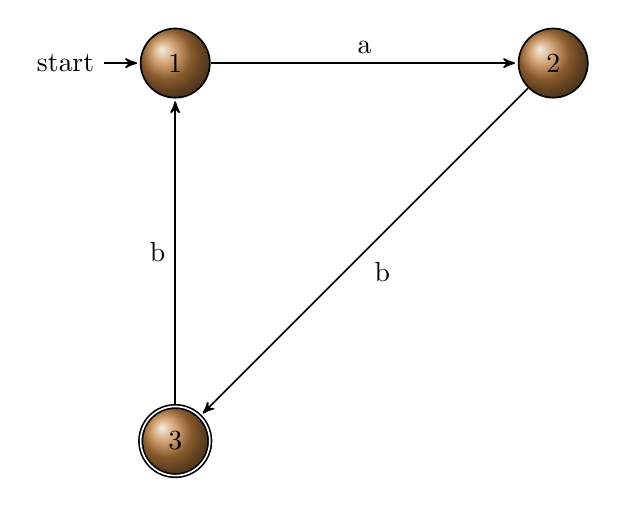
\begin{tikzpicture}[->,>=stealth',shorten >=1pt,auto,node distance=4.8cm, semithick]
\tikzstyle{every state}=[draw=black,text=black, ball color=brown]
\node[initial,state] (1) {1};
\node[state][right of=1](2){2};
\node[state, accepting][below of=1](3){3};
\path (1)edge node{a}(2)
          (2)edge node{b}(3)
          (3)edge node{b}(1);       
\end{tikzpicture} 
\end{center}
\end{figure}
%2
\section{}
\begin{enumerate}
\item Palindromes
\begin{proof}
For any regular language L, there exists a number p such that for any string w in L of length at least p there are strings x,y,z such that
\begin{enumerate}
\item If w = xyz.
\item And if x = a, y = b, z = a.
\item or if x = b, y = a, z = b.
\item Then $w = a^{90 + 1}ba^{90}$
\item and $w = b^{90 + 1}ab^{90}$
\item Therefore Palindromes are nonregular
\end{enumerate}
\end{proof}
\item Equal
\begin{proof}
For any regular language L, there exists a number p such that for any string w in L of length at least p there are strings x,y,z such that
\begin{enumerate}
\item  EQUAL = $\{\Lambda \quad ab \quad ba \quad aabb \quad abab \quad abba \quad baab \quad baba \quad bbaa \quad aaabbb...\}$
\item $\{a^nb^n\} = \mathbf{a^*b^*} \cap EQUAL$
\item If $a^*b^*$ is regular then so is the result of $\mathbf{a^*b^*} \cap EQUAL$
\item $w =  xyz$
\item $\mid xy \mid \le  p$
\item $\mid y \mid \ge 1$
\item Then $x = a^n, y = a^2, z = b^n$
\item So then xyyz would allow aaab which is not in this language.
\item Therefore this language is nonregular
\end{enumerate}
\end{proof}
\end{enumerate}
%3
\section{}
Prove that the below generates the language defined by the regular expression: $\mathbf{a^*bb}$
$$\mathbf {Prod 1 \quad S \to aS \mid bb}$$
\begin{equation}
\begin{split}
&S \Longrightarrow aS\\
&\Longrightarrow aaS\\
&\Longrightarrow aaaS\\
&\Longrightarrow aaaaS\\
&\Longrightarrow aaaaaS\\
&\Longrightarrow aaaaabb\\
\end{split}
\end{equation}
This derivation could continue infinitely until terminal bb is appended.
%4
\section{}
To generate aabbab using: $a(a +b)*$
\begin{equation}
\begin{split}
&\mathbf {Prod 1 \quad S \to aX}\\
&\mathbf{Prod 2 \quad X \to aX \mid bX \mid \Lambda}\\
&S \Longrightarrow aX \quad \text{(by Prod 1)}\\
&\Longrightarrow aaX \quad \text{(by Prod 2)}\\
&\Longrightarrow aabX \quad \text{(by Prod 2)}\\
&\Longrightarrow aabbX \quad \text{(by Prod 2)}\\
&\Longrightarrow aabbaX \quad \text{(by Prod 2)}\\
&\Longrightarrow aabbabX \quad \text{(by Prod 2)}\\
&\Longrightarrow aabbab\Lambda \quad \text{(by Prod 2)}\\
\end{split}
\end{equation}
%5
\section{}
To generate bbabaaa using: $(a + b)^*a(a + b)^*a(a + b)^*$
\begin{equation}
\begin{split}
&\mathbf {Prod 1 \quad S \to XaXaX}\\
&\mathbf {Prod 2 \quad X \to aX \mid bX \mid \Lambda}\\
&S \Longrightarrow XaXaX \quad \text{(by Prod 1)}\\
&\Longrightarrow XaXaaX \quad \text{(by Prod 2)}\\
&\Longrightarrow bXaXaaX \quad \text{(by Prod 2)}\\
&\Longrightarrow bXaXaa \quad \text{(by Prod 2)}\\
&\Longrightarrow bXabXaa \quad \text{(by Prod 2)}\\
&\Longrightarrow bXabaXaa \quad \text{(by Prod 2)}\\
&\Longrightarrow bbXabaXaa \quad \text{(by Prod 2)}\\
&\Longrightarrow bbabaXaa \quad \text{(by Prod 2)}\\
&\Longrightarrow bbabaaa \quad \text{(by Prod 2)}\\
\end{split}
\end{equation}
%6
\section{}
\begin{equation}
\begin{split}
&\mathbf {Prod 1 \quad S \to Xa}\\
&\mathbf {Prod 2 \quad X \to bbX \mid bbS \mid bb\mid\Lambda}\\
\end{split}
\end{equation}
\clearpage
%7
\section{}
%sub1
\subsection{}
This CFG cannot match aaaa, abaa, or bbaa as it will always be abab:
\begin{equation}
\begin{split}
&\mathbf {Prod 1 \quad S \to aSb \mid ab}\\
\end{split}
\end{equation}
\begin{tikzpicture}[level 1/.style={sibling distance=6em},
                   level 2/.style={sibling distance=1em}, level distance=2cm]]
\node {S}
child {node {aSb} child {node {ab}}}
child {node {ab}}
;
\end{tikzpicture} 
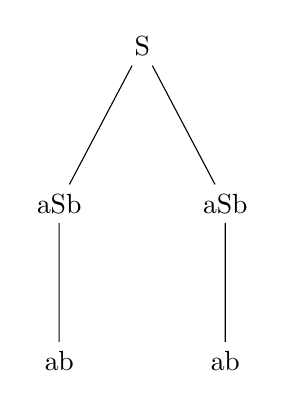
\begin{tikzpicture}[level 1/.style={sibling distance=6em},
                   level 2/.style={sibling distance=1em}, level distance=2cm]]
\node {S}
child {node {aSb} child {node {ab}}}
child {node {aSb} child {node {ab}}}
;
\end{tikzpicture} 
\begin{tikzpicture}[level 1/.style={sibling distance=6em},
                   level 2/.style={sibling distance=1em}, level distance=2cm]]
\node {S}
child {node {ab}}
child {node {aSb} child {node {ab}}}
;
\end{tikzpicture} 
%sub2
\subsection{}
This CFG can create the string aaaa:
\begin{equation}
\begin{split}
&\mathbf {Prod 1 \quad S \to aS \mid bS \mid a}\\
\end{split}
\end{equation}
\begin{tikzpicture}[level 1/.style={sibling distance=6em},
                   level 2/.style={sibling distance=1em}, level distance=2cm]]
\node {S}
child {node {aS}child {node {a}}child {node {a}}}
child {node {bS}child {node {a}}child {node {a}}}
child {node {a}}
;
\end{tikzpicture} 

\clearpage
%sub3
\subsection{}

\begin{equation}
\begin{split}
&\mathbf {Prod 1 \quad S \to aS \mid aSb \mid X}\\
&\mathbf {Prod 2 \quad X \to aXa \mid a}\\
\end{split}
\end{equation}
\begin{tikzpicture}[level 1/.style={sibling distance=6em},
                   level 2/.style={sibling distance=1em}, level distance=2cm]]
\node {S}
child {node {aS}}
child {node {aSb}}
child {node {X}}

;
\end{tikzpicture} 
%sub4
\subsection{}
\begin{equation}
\begin{split}
&\mathbf {Prod 1 \quad S \to aAS \mid a}\\
&\mathbf {Prod 2 \quad A \to SbA \mid SS \mid ba}\\
\end{split}
\end{equation}
\begin{tikzpicture}[level 1/.style={sibling distance=6em},
                   level 2/.style={sibling distance=1em}, level distance=2cm]]
\node {S}
child {node {}}

;
\end{tikzpicture} 
%sub5
\subsection{}
\begin{equation}
\begin{split}
&\mathbf {Prod 1 \quad S \to aB \mid bA}\\
&\mathbf {Prod 2 \quad A \to a \mid aS \mid bAA}\\
&\mathbf{Prod 3 \quad B \to b \mid bS \mid aBB}\\
\end{split}
\end{equation}
\begin{tikzpicture}[level 1/.style={sibling distance=6em},
                   level 2/.style={sibling distance=1em}, level distance=2cm]]
\node {S}
child {node {}}

;
\end{tikzpicture} 
\clearpage
%8
\section{}
%9
\section{}
%10
\section{}
%11
\section{}
\end{document}